\chapter{\selectlanguage{greek}Γραμμικοί Μπλoκ Κώδικες}\externaldocument{chapter1.tex}
Στο κεφάλαιο αυτό, παρουσιάζονται οι βασικές αλγεβρικές δομικές ιδιότητες που προσδίδονται στους κώδικες καναλιού, οι οποίες διακρίνουν και τους κώδικες πάνω στους οποίους στηρίζεται η παρούσα εργασία και που θα παρουσιαστούν στο επόμενο κεφάλαιο. Όπως αναφέρθηκε στο εισαγωγικό κεφάλαιο, το σώμα που υιοθετείται είναι το $\mathbb{F}_2$. Συνεπώς, θεωρείται πως η έξοδος της πηγής πληροφορίας είναι μια διακριτή ακολουθία \en{i.i.d.} δυαδικών ψηφίων, η οποία καλείται \textit{ακολουθία πληροφορίας}. Η μετάδοση λαμβάνει χώρα μέσω του διακριτού καναλιού, όπως αυτό ορίστηκε στον Ορισμό \ref{def:discrete channel}. Υπενθυμίζεται ακόμη πως η έκφραση \enquote{κώδικας $C(n,M)$}, αναφέρεται στο κωδικό βιβλίο του κώδικα.

\section{\en{Block} κώδικες}
Ξεκινώντας τη μελέτη των δομών που αναφέρθηκαν παραπάνω, ορίζεται η υποομάδα των κωδίκων καναλιού, οι κώδικες \textit{\en{block}} (\en{block codes}).

Η αρχή λειτουργίας της \en{block} κωδικοποίησης, συνίσταται στην κατάτμηση της ακολουθίας πληροφορίας σε σταθερά \en{block} $\mathbf{u} = (u_0, u_1, ..., u_{k-1})$ μήκους $k$ και στην απεικόνισή της στην είσοδο του καναλιού, μέσω του κωδικοποιητή καναλιού, στην κωδική λέξη $\mathbf{v} = (v_0, v_1, ..., v_{n-1})$ μήκους $n$, με $n>k$. H απεικόνιση αυτή είναι ανεξάρτητη από τα προηγούμενα \en{block}, δηλαδή δεν υπάρχει μνήμη από ένα \en{block} μήνυμα, σε ένα άλλο επόμενο \cite{proakis1994communication}.

\begin{figure}[h]
\center{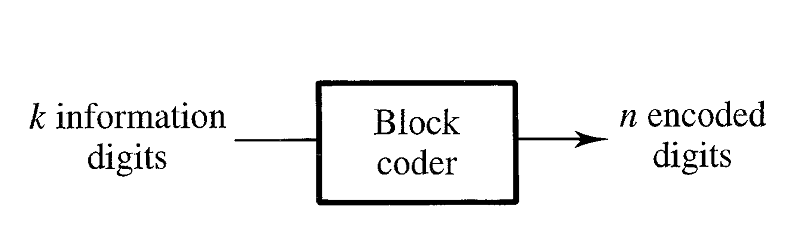
\includegraphics[width=0.75\linewidth]{figures/linear_block_codes.png}}
\caption{Σχηματικό διάγραμμα ενός \en{block} κώδικα}
\label{fig:linear block codes}
\end{figure}

\subsection{Ρυθμός κώδικα}
Στο προηγούμενο κεφάλαιο ορίστηκε ο ρυθμός του κώδικα ως $R=\frac{\log_{2}M}{n}$. Επίσης ισχύει πως η πληθυκότητα (\en{cardinality}) του \en{block} κώδικα $C$ στο $\mathbb{F}_2$, το σύνολο δηλαδή των δυνατών κωδικών λέξεων του κωδικού βιβλίου, είναι $M=2^k$. Εφαρμόζοντας τις παραπάνω σχέσεις, προκύπτει ο λόγος
\begin{equation}
R = \frac{\log_{2}2^{k}}{n} = \frac{k}{n}
\label{eq:code rate}
\end{equation}
ο οποίος καλείται \textit{ρυθμός} του \en{block} κώδικα $C$ (\en{\textit{code rate}}) και αντιπροσωπεύει τον μέσο όρο πληροφορίας που αποστέλλεται με κάθε κωδικό \en{bit}, ανν τα \en{bits} πληροφορίας είναι ανεξάρτητα και ισοπίθανα (\en{i.i.d.}). Προφανώς ισχύει $0<R<1$.

\vspace{5mm}

Όπως αναφέρθηκε, ο κώδικας αντιστοιχίζει κάθε μήνυμα πληροφορίας $\mathbf{u}$, στην κωδικολέξη $\mathbf{v}$, μήκους $n$, με $n>k$. Tα $n-k$ επιπλέον \en{bits} που προστίθενται στο μήνυμα από τον κωδικοποιητή καναλιού καλούνται \textit{πλεονασματικά} (\en{redundant}) \en{bits}.

Τα πλεονασματικά \en{bits} δεν περιέχουν επιπλέον πληροφορία και ο σκοπός τους είναι να δώσουν δυνατότητες \textit{ανίχνευσης} και \textit{διόρθωσης} σφαλμάτων, που προκύπτουν κατά τη μετάδοση στο κανάλι, λόγω θορύβου ή/και παρεμβολών. Το πως διαμορφώνονται αυτά τα πλεονασματικά \en{bits}, ώστε ο \en{block} κώδικας $C(n,k)$ να έχει ικανοποιητικές δυνατότητες ανίχνευσης ή/και διόρθωσης, αποτελεί μείζων ζήτημα της σχεδίασης μηχανισμών κωδικοποίησης \cite{ryan2009channel}.

\section{Γραμμικοί \en{block} κώδικες}
Για ένα \en{block} κώδικα $C(n,M)$, με $2^k$ κωδικές λέξεις και χωρίς περεταίρω δομή, έχει ήδη αναφερθεί πως ο μηχανισμός κωδικοποίησης απαιτείται να καταχωρεί τις $2^k$ κωδικές αυτές λέξεις σε ένα κωδικό λεξικό και ο μηχανισμός αποκωδικοποίησης -μεταξύ άλλων- να κάνει αναζήτηση σε ένα πίνακα $2^k\times{n}$, ώστε να αποφασίσει για τη μεταδιδόμενη κωδική λέξη.

Επομένως, επιπρόσθετα από την δόμηση σε κωδικά \en{blocks}, είναι αναγκαίο να προσδώσουμε επιπλέον δομικές ιδιότητες στον κώδικα $C(n,M)$, ώστε οι παραπάνω διαδικασίες να καταστούν πρακτικά υλοποιήσιμες. Μια τέτοια επιθυμητή δομική ιδιότητα ώστε ο \en{block} κώδικας να είναι υλοποιήσιμος με πρακτικό τρόπο, είναι η \textit{γραμμικότητα}.

\vspace{5mm}

\begin{definition}
Ένας δυαδικός κώδικας μήκους $n$ καλείται $(n,k)$ \textit{γραμμικός \en{block} κώδικας}, ανν οι $2^k$ κωδικές του λέξεις σχηματίζουν έναν $k$-διάστατο υποχώρο του δυανυσματικού χώρου $V$ όλων των δυνατών $n$-άδων στο $\mathbb{F}_2$ \cite{ryan2009channel}.
\label{def:linear block code}
\end{definition}

Ένας ισοδύναμος ορισμός είναι ο εξής:

\begin{definition}
Ένας κώδικας \en{block} είναι γραμμικός αν κάθε γραμμικός συνδυασμός δύο κωδικών του λέξεων, είναι επίσης κωδική του λέξη. Στο $\mathbb{F}_2$, αν $\mathbf{c_i}$ και $\mathbf{c_j}$ οι δύο κωδικές λέξεις, τότε πρέπει $\mathbf{c_i}\oplus\mathbf{c_j}$ να είναι επίσης κωδική λέξη του $C$, όπου με $\oplus$ συμβολίζεται η συνιστώσα-προς-συνιστώσα \en{modulo-2} πρόσθεση \cite{proakis1994communication}.
\end{definition}

Φαίνεται επομένως πως ένας (δυαδικός) \en{block} κώδικας είναι γραμμικός, ανν υπάρχει \enquote*{1-1} αντιστοιχία μεταξύ του μηνύματος \en{\textbf{u}} και της κωδικολέξης \en{\textbf{v}}. Επίσης, η ακολουθία \textbf{0} αποτελεί κωδική λέξη κάθε γραμμικού \en{block} κώδικα, αφού μπορεί να προκύψει ως συνιστώσα-προς-συνιστώσα \en{modulo-2} πρόσθεση μιας κωδικής λέξης με τον εαυτό της. Ακόμη φαίνεται πως η γραμμικότητα ενός κώδικα εξαρτάται αποκλειστικά από τις κωδικές του λέξεις και όχι από τον τρόπο με τον οποίο η ακολουθία πληροφορίας απεικονίζεται σε αυτές.

\section{Αναπαράσταση σε πίνακα}

\subsection{Πίνακας \en{G}}
Σύμφωνα με τον ορισμό του γραμμικού \en{block} κώδικα $C(n,k)$, αποδεικνύεται πως υπάρχουν $k$ γραμμικά ανεξάρτητες κωδικές λέξεις, $\mathbf{g_0, g_1, ..., g_{k-1}}$, έτσι ώστε κάθε κωδική λέξη $\mathbf{v}$ να προκύπτει ως γραμμικός συνδυασμός τους. Οι $k$ γραμμικά ανεξάρτητες αυτές κωδικές λέξεις λέγεται ότι σχηματίζουν μια \textit{βάση} του $C$.

Με βάση αυτό, η κωδική λέξη προκύπτει ως εξής: έστω $\mathbf{u} = (u_0, u_1, ..., u_{k-1})$ το μήνυμα στην είσοδο του κωδικοποιητή. Η κωδικολέξη $\mathbf{v} = (v_0, v_1, ..., v_{n-1})$ δίνεται από τον γραμμικό συνδυασμό των $\mathbf{g_0, g_1, ..., g_{k-1}}$ με συντελεστές τα $k$ \en{bits} πληροφορίας, από την παρακάτω εξίσωση:

\begin{equation}
\mathbf{v}=u_0\mathbf{g_0}+u_1\mathbf{g_1}+...+u_{k-1}\mathbf{g_{k-1}}
\label{eq:codeword formation}
\end{equation}

Οι συνιστώσες των $k$ γραμμικά ανεξάρτητων κωδικολέξεων μπορούν να αναπαρασταθούν ως γραμμές ενός $k\times n$ πίνακα στο $\mathbb{F}_2$ ως εξής:

\begin{equation}
\mathbf{G}=\begin{bmatrix}\mathbf{g_0}\\\mathbf{g_1}\\\vdots\\\mathbf{g_{k-1}}\\\end{bmatrix}=\begin{bmatrix}g_{0,0} & g_{0,1} & \cdots & g_{0,n-1}\\g_{1,0} & g_{1,1} & \cdots & g_{1,n-1}\\\vdots & \vdots & \ddots & \vdots\\g_{k-1,0} & g_{k-1,1} & \cdots & g_{k-1,n-1}\\\end{bmatrix}
\label{eq:generator matrix}
\end{equation}

Σε αυτή την περίπτωση, η κωδικολέξη $\mathbf{v}$ που αντιστοιχεί στο μήνυμα $\mathbf{u}$, δίνεται από τον πολλαπλασιασμό πινάκων: 

\begin{equation}
\mathbf{v=u \cdot G}
\label{eq:check equation}
\end{equation}

Ο πίνακας \en{\textbf{G}} καλείται \textit{πίνακας γεννήτορας} \en{(generator matrix)} του $(n,k)$ γραμμικού \en{block} κώδικα $C$. Γενικά, ένας γραμμικός \en{block} κώδικας δεν έχει μοναδική βάση. Συνεπώς κάθε επιλογή βάσης του $C$ δίνει διαφορετικό γεννήτορα πίνακα, οπότε προκύπτει πως ο πίνακας \en{\textbf{G}} δεν είναι μοναδικός για δεδομένο κώδικα. Ο βαθμός (\en{rank}) του πίνακα \en{\textbf{G}} είναι προφανώς ίσος με τη διάσταση του κώδικα $C$.

Παρατηρείται συνεπώς, πως μειώνεται σημαντικά η πολυπλοκότητα περιγραφής του κώδικα, αφού πλέον αρκέι ο κωδικοποιητής να αποθηκεύσει τις $k$ γραμμές του πίνακα \en{\textbf{G}}. Επιπρόσθετα, η εκτέλεση του πολλαπλασιασμού πινάκων που περιγράφει η \ref{eq:check equation} απαιτεί περίπου $kn$ πράξεις, δηλαδή είναι τετραγωνικής πολυπλοκότητας ως προς το $n$ - $\mathcal{O}(n^2)$.

\subsection{Πίνακας \en{H}}
\begin{definition}
Ο δυικός κώδικας (\en{\textit{dual code}}) του $C$, $C_d$ δίνεται από τις παρακάτω $n$-άδες:$$C_d=\lbrace\mathbf{w}\in V:\langle \mathbf{w,v} \rangle =0\;\;\;\forall\;\mathbf{v}\in C\rbrace$$,
όπου με $\langle\cdot,\cdot\rangle$ συμβολίζεται το διανυσματικό εσωτερικό γινόμενο \cite{ryan2009channel}.
\label{def:dual code}
\end{definition}

Από τον Ορισμό \ref{def:dual code} προκύπτουν τα παρακάτω:

\begin{itemize}
\item Αν η βάση του $C$ αποτελείται από $k$ γραμμικά ανεξάρτητες κωδικές λέξεις, η βάση του $C_d$ αποτελείται από ($n-k$) γραμμικά ανεξάρτητες $n$-άδες.
\item Έστω $\mathbf{h_0, h_1, ..., h_{n-k-1}}$ οι ($n-k$) αυτές, γραμμικά ανεξάρτητες $n$-άδες. Συνεπάγεται πως κάθε $n$-άδα στον $C_d$ προκύπτει ως γραμμικός συνδυασμός τους
\item Ομοίως με τον πίνακα \en{\textbf{G}}, οι παραπάνω γραμμικά ανεξάρτητες $n$-άδες μπορούν να αναπαρασταθούν ως γραμμές ενός πίνακα στο $\mathbb{F}_2$, που σχηματίζεται ως εξής:

\begin{equation}
\mathbf{H}=\begin{bmatrix}\mathbf{h_0}\\\mathbf{h_1}\\\vdots\\\mathbf{h_{n-k-1}}\\\end{bmatrix}=\begin{bmatrix}h_{0,0} & h_{0,1} & \cdots & h_{0,n-1}\\h_{1,0} & h_{1,1} & \cdots & h_{1,n-1}\\\vdots & \vdots & \ddots & \vdots\\h_{n-k-1,0} & h_{n-k-1,1} & \cdots & h_{n-k-1,n-1}\\\end{bmatrix}
\label{eq:parity check matrix}
\end{equation}
\item Ο πίνακας $\mathbf{H}$ είναι γεννήτορας πίνακας του $C_d$, ακριβώς όπως ο $\mathbf{G}$ είναι του $C$. Λόγω αυτού και από την ιδιότητα της ορθογωνιότητας, προκύπτει η πολύ χρήσιμη εξίσωση $\mathbf{G} \cdot \mathbf{H^T} = \mathbf{0}$, όπου $\mathbf{0}$ μηδενικός $k \times (n-k)$ πίνακας.
\end{itemize}

Ακόμη, προκύπτει πως ο κώδικας $C$ ορίζεται με μοναδικό τρόπο από τον πίνακα $\mathbf{H}$, επειδή κάθε δυαδική $n$-άδα $\mathbf{v}$ είναι κωδικολέξη του $C$ ανν
ισχύει $\mathbf{v} \cdot \mathbf{H^T} = \mathbf{0}$, δηλαδή
\begin{equation}
C=\lbrace\mathbf{v}\in V:\mathbf{v} \cdot \mathbf{H^T} = \mathbf{0}\rbrace
\label{eq:decoding equation}
\end{equation}

Ο πίνακας $\mathbf{H}$ καλείται πίνακας \textit{ελέγχου ισοτιμίας} (\en{parity check matrix}) του κώδικα $C$. Από την παραπάνω σχέση ορισμού ενός γραμμικού κώδικα (εξίσωση \ref{eq:decoding equation}), προέρχεται και το όνομα του $\mathbf{H}$, αφού, στην πλευρά του αποκωδικοποιητή, ο $\mathbf{H}$ χρησιμοποιείται για την επαλήθευση του παραπάνω συστήματος ομογενών εξισώσεων, όταν το διάνυσμα $\mathbf{v}$, αντικατασταθεί με το ληφθέν διάνυσμα.

Παρατηρείται επομένως, πως ο γραμμικός \en{block} κώδικας $C$ μπορεί να οριστεί πλήρως από δύο πίνακες, τον γεννήτορα και τον πίνακα ελέγχου ισοτιμίας. Στη γενική περίπτωση, η κωδικοποίηση του $C$ βασίζεται στον γεννήτορα πίνακα και ακολουθεί την εξίσωση \ref{eq:check equation}, ενώ η αποκωδικοποίηση βασίζεται στον πίνακα ελέγχου ισοτιμίας.

Ο πίνακας ελέγχου ισοτιμίας μπορεί να περιγράψει πλήρως έναν κώδικα, και πολλές κατηγορίες γραμμικών \en{block} κωδίκων κατασκευάζονται με βάση τον πίνακα $\mathbf{H}$. Ο πίνακας $\mathbf{H}$ είναι σε μορφή \textit{πλήρους βαθμού} (\en{full rank}), ανν ο βαθμός του είναι ίσος με το πλήθος των σειρών. Σε πολλές περιπτώσεις, ο πίνακας $\mathbf{H}$ δεν δίνεται σε \en{full rank} μορφή, δηλαδή το πλήθος των σειρών του είναι μεγαλύτερο από το \en{rank} του, $n-k$, ή ισοδύναμα, ορισμένες από τις σειρές του είναι γραμμικός συνδυασμός των $n-k$ γραμμικά ανεξάρτητων σειρών. Οι σειρές αυτές ονομάζονται \textit{πλεονάζουσες} (\en{redundant}) σειρές. 

Οι κώδικες Πίνακα Ισοτιμίας Χαμήλης Πυκνότητας (\en{Low Density Parity Check - LDPC}), που θα εξεταστούν στη συνέχεια της εργασίας, διακρίνονται από πίνακες $\mathbf{H}$ που δεν είναι \en{full rank} \cite{cover2012elements}, \cite{ryan2009channel}.

\section{Κώδικες σε συστηματική μορφή}

\begin{figure}[h]
\center{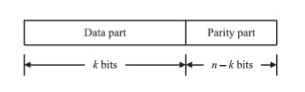
\includegraphics[width=0.65\linewidth]{figures/systematic_form.png}}
\caption{Κωδική λέξη σε συστηματική μορφή}
\label{fig:systematic form}
\end{figure}

Μία ακόμη επιθυμητή ιδιότητα, είναι οι κωδικές λέξεις ενός γραμμικού \en{block} κώδικα $C(n,k)$ να έχουν τη μορφή που φαίνεται στο Σχήμα \ref{fig:systematic form}, η οποία καλείται \textit{συστηματική μορφή} (\en{systematic form}). Στη συστηματική μορφή, η κωδική λέξη χωρίζεται στο τμήμα μηνύματος (\en{data part}) και στο πλεονάζον τμήμα ελέγχου (\en{parity part}). Το τμήμα μηνύματος αποτελείται από τα $k$ αναλλοίωτα ψηφία πληροφορίας και το πλεονάζον τμήμα ελέγχου, από τα $n-k$ \en{bits} ελέγχου ισοτιμίας. Ολόκληρος ο γραμμικός \en{block} κώδικας $C(n,k)$ βρίσκεται σε \textit{συστηματική} μορφή, όταν όλα τα στοιχεία του κωδικού βιβλίου βρίσκονται σε συστηματική μορφή, ή ισοδύναμα, όταν μπορέι να οριστεί πλήρως από έναν $k \times n$ γεννήτορα πίνακα με την παρακάτω μορφή:

\begin{equation}
\mathbf{G} = \left[\mathbf{P}\;\;\mathbf{I}_{k}\right]= 
\left[\underbrace{\begin{matrix}
p_{0,0} & p_{0,1} & \cdots & p_{0,n-k-1} \\
p_{1,0} & p_{1,1} & \cdots & p_{1,n-k-1} \\
\vdots & \vdots & \ddots & \vdots \\
p_{k-1,0} & p_{k-1,1} & \cdots & p_{k-1,n-k-1}
\end{matrix}}_{\text{\en{\textbf{P}} πίνακας}}\;
\underbrace{\begin{matrix}
1 & 0 & \cdots & 0 \\
0 & 1 & \cdots & 0 \\
\vdots & \vdots & \ddots & \vdots \\
0 & 0 & \cdots & 1
\end{matrix}}_{\text{$k\times k$ $\mathbf{I}_k$ μοναδιαίος πίνακας}}\right]
\label{eq:generator matrix systematic form}
\end{equation}

\vspace{5mm}

Όπως διαπιστώνεται και από την εξίσωση \ref{eq:generator matrix systematic form}, ο γεννήτορας πίνακας $\mathbf{G}$, που για συντομία σημειώνεται ως $\mathbf{G}=\left[\mathbf{P}\;\;\mathbf{I}_k\right]$, αποτελείται από δύο υποπίνακες, έναν $k\times (n-k)$ υποπίνακα $\mathbf{P}$ στα αριστερά, ο οποίος καλείται υποπίνακας ελέγχου ισοτιμίας του $\mathbf{G}$ και έναν $k\times k$ μοναδιαίο πίνακα $\mathbf{I}_k$ στα δεξιά \cite{ryan2009channel}.

Η συστηματική μορφή του πίνακα $\mathbf{G}$ έχει σημαντικά πλεονεκτήματα καθώς σε κάθε κωδική λέξη, τα \en{bits} πληροφορίας παραμένουν αναλλοίωτα στις αρχικές $k$ θέσεις της. Μειώνεται συνεπώς η πολυπλοκότητα κωδικοποίησης, αφού χρειάζεται να υπολογιστούν μόνο τα σύμβολα στις θέσεις του πλεονάζοντος τμήματος ελέγχου.

Αντίστοιχα, η συστηματική μορφή του πίνακα ελέγχου ισοτιμίας διαμορφώνεται ως εξής:

\begin{equation}
\mathbf{H}=\left[\mathbf{I}_{n-k}\;\;\mathbf{P^T}\right]
=\begin{bmatrix}
1 & 0 & \cdots & 0 & \; & p_{0,0} & p_{1,0} & \cdots & p_{k-1,0} \\
0 & 1 & \cdots & 0 & \; & p_{0,1} & p_{1,1} & \cdots & p_{k-1,1} \\
\vdots & \vdots & \ddots & \vdots  & \; & \vdots & \vdots & \ddots & \vdots \\
0 & 0 & \cdots & 1 & \; & p_{0,n-k} & p_{1,n-k} & \cdots & p_{k-1,n-k}
\end{bmatrix}
\label{eq:parity check matrix systematic form}
\end{equation}

\vspace{5mm}
Προφανώς ισχύει και πάλι ότι $\mathbf{G}\cdot\mathbf{H^T}=\mathbf{0}$.

Θεωρείται και πάλι το μήνυμα πληροφορίας $\mathbf{u} = (u_0, u_1, ..., u_{k-1})$. Αν εφαρμοστεί η εξίσωση \ref{eq:check equation}, όταν ο πίνακας $\mathbf{G}$ είναι σε συστηματική μορφή, η κωδική λέξη προκύπτει από τον παρακάτω πολλαπλασιασμό:

\begin{equation}
\begin{split}
\mathbf{v} & = \left( u_0, u_1, \cdots, u_{k-1} \right) \cdot \mathbf{G}\\
& = \left( v_0, v_1, \cdots, v_{n-k-1}, v_{n-k}, \cdots, v_{n-1} \right)
\end{split}
\label{eq:systematic codeword formation}
\end{equation}

\vspace{5mm}

τα $n$ στοιχεία της οποίας προκύπτουν ως εξής:

\begin{equation}
\begin{aligned}
v_{n-k+i}=u_i\;\;\ & \forall\;\;0\leq i < k  \\
v_j=u_0p_{0,j}+u_1p_{1,j}+\cdots+u_{k-1}p_{k-1,j}\;\; & \forall\;\;0\leq j < n-k
\end{aligned}
\label{eq:systematic codeword bits}
\end{equation}

\vspace{5mm}

Οι εξισώσεις \ref{eq:systematic codeword bits} δείχνουν πως τα δεξιότερα $k$ \en{bits} της κωδικής λέξης παραμένουν αναλλοίωτα τα $k$ \en{bits} του μηνύματος πληροφορίας και τα υπόλοιπα $n-k$ αποτελούν γραμμικό συνδυασμό των \en{bits} πληροφορίας και ορίζονται πλήρως από τις $n-k$ στήλες του υποπίνακα $\mathbf{P}$, όπως αυτός ορίζεται στην εξίσωση \ref{eq:generator matrix systematic form}. Η δεύτερη έκφραση, αποτελέι ένα σύστημα $n-k$ εξισώσεων οι οποίες ονομάζονται εξισώσεις ελέγχου ισοτιμίας.

Επίσης φανερώνονται τα πλεονεκτήματα που προσφέρει η συστηματική μορφή. Λιγότερων υπολογισμών, καθώς το μήνυμα πληροφορίας παραμένει ατόφιο και 
απαιτείται υπολογισμός μόνο των \en{bits} του τμήματος ελέγχου, κάτι που οδηγεί σε μειωμένη πολυπλοκότητα περιγραφής και κωδικοποίησης-αποκωδικοποίησης.

\section{Κατανομή Βαρών - Ελάχιστη Απόσταση \en{Hamming}}

Παρακάτω θα δωθούν οι ορισμοί μερικών βασικών παραμέτρων ενός κώδικα. Οι έννοιες που θα οριστούν, βοηθούν στην κατανόηση της δυνατότητας εντοπισμού και διόρθωσης σφαλμάτων των γραμμικών \en{block} κωδίκων που θα συζητηθεί στη συνέχεια.

\begin{definition}Απόσταση \en{Hamming}

Έστω δύο δυαδικές $n$-άδες, $\mathbf{v}$ και $\mathbf{w}$. Η απόσταση \en{Hamming} ορίζεται ως ο αριθμός των συνιστωσών στις οποίες διαφέρουν μεταξύ τους και συμβολίζεται με $d\left(\mathbf{v},\mathbf{w}\right)$.
\label{def:Hamming distance}
\end{definition}

\begin{definition}Βάρος \en{Hamming}

Το βάρος \en{Hamming} μιας δυαδικής $n$-άδας, $\mathbf{v}$ ορίζεται ως το πλήθος των μη μηδενικών στοιχείων της και συμβολίζεται με $w\left(\mathbf{v}\right)$
\label{def:Hamming weight}
\end{definition}

Από τους ορισμούς \ref{def:Hamming distance}, \ref{def:Hamming weight} προκύπτει πως η απόσταση \en{Hamming} μεταξύ δύο $n$-άδων ισούται με το βάρος του αθροίσματός τους \en{modulo}-2, δηλ $d\left(\mathbf{v},\mathbf{w}\right) = w\left(\mathbf{v}+\mathbf{w}\right)$.

\begin{definition}
Η ελάχιστη απόσταση ενός κώδικα ορίζεται ως η ελάχιστη απόσταση \en{Hamming} μεταξύ δύο διαφορετικών κωδικών λέξεων, δηλαδή
\begin{equation}
d_{min} = \min_{\mathbf{v}, \mathbf{w}}d\left(\mathbf{v}, \mathbf{w}\right)
\label{eq:min distance}
\end{equation}
\end{definition}

\begin{definition}
Το ελάχιστο βάρος ενός κώδικα, ορίζεται από την παρακάτω σχέση
\begin{equation}
w_{min} = \min_{\mathbf{v}\neq\mathbf{0}}w\left(\mathbf{v}\right)
\label{eq:min weight}
\end{equation}
είναι δηλαδή, το ελάχιστο των βαρών των κωδικών λέξεων του κώδικα, αν εξαιρεθεί η μηδενική κωδική λέξη.
\end{definition}

Από τα παραπάνω προκύπτει το παρακάτω θεώρημα:

\begin{theorem}
Η ελάχιστη απόσταση ενός κώδικα $d_{min}$ είναι ίση με το ελάχιστο βάρος ενός κώδικα $w_{min}$. Η απόδειξη του θεωρήματος είναι η ακόλουθη:
\begin{equation}
\begin{split}
d_{min}(C) & = \min \lbrace d \left( \mathbf{v},\mathbf{w} \right) : \mathbf{v},\mathbf{w} \in C, \mathbf{v}\neq\mathbf{w} \rbrace \\
& = \min \lbrace w \left( \mathbf{v}+\mathbf{w} \right) : \mathbf{v},\mathbf{w} \in C, \mathbf{v}\neq\mathbf{w} \rbrace \\
& = \min \lbrace w \left( \mathbf{x} \right) : \mathbf{x} \in C, \mathbf{x}\neq\mathbf{0} \rbrace \\
& = w_{min}(C).
\end{split}
\end{equation}
\label{theorem:min distance}
\end{theorem}

Τέλος, δίνεται το παρακάτω θεώρημα, χωρίς απόδειξη:

\begin{theorem}
Έστω γραμμικός \en{block} κώδικας $C(n,k)$ με πίνακα ελέγχου ισοτιμίας $\mathbf{H}$.
\begin{itemize}
\item Για κάθε κωδική λέξη του $C$ με βάρος $i$, υπάρχουν ακριβώς $i$ στήλες του πίνακα $\mathbf{H}$, των οποίων το διανυσματικό άθροισμα είναι το μηδενικό διάνυσμα στήλη και αντιστρόφως.
\item Το ελάχιστο βάρος (ελάχιστη απόσταση) του $C$ είναι ίσο με το μικρότερο αριθμό στηλών του $\mathbf{H}$ που έχουν διανυσματικό άθροισμα μηδέν, δηλαδή είναι γραμμικά ανεξάρτητες.
\item Η ελάχιστη απόσταση (ελάχιστο βάρος) του $C$ είναι τουλάχιστον $d$, ανν δεν υπάρχουν $d-1$ ή λιγότερες στήλες με διανυσματικό άθροισμα μηδέν.
\end{itemize}
\label{theorem:distance weight parity check matrix}
\end{theorem}
\cite{ryan2009channel}, \cite{peterson1972error}.

\vspace{3mm}
Μπορεί πλέον να οριστεί και η \textit{κατανομή βάρους} του κώδικα $C$. Έστω $A_i$ ο αριθμός των κωδικών λέξεων του $C(n,k)$ με βάρος \en{Hamming} $i$. Η κατανομή βάρους του $C$ αποτελείται από τους αριθμούς $A_0,A_1,\cdots,A_n$ για $0\leq i \leq n$. Ισχύουν οι παρακάτω σχέσεις:

\begin{equation}
\begin{aligned}
A_0+A_1+\cdots+A_n& = 2^k \\ 
Α_0 & =  1
\end{aligned}
\end{equation}

Η κατανομή βάρους ενός κώδικα αποτελεί σημαντικό εργαλείο στον καθορισμό της πιθανότητας να συμβεί ένα μη-ανιχνεύσιμο σφάλμα κατά την αποκωδικοποίηση καθώς αποτελεί παράγοντα του άνω ορίου της πιθανότητας αυτής. Δίνει επίσης την εικόνα της κατανομής αποστάσεων μεταξύ των κωδικών λέξεων ενός κώδικα, σε σχέση με την κωδική λέξη $\mathbf{0}$, καθώς το $A_i$ αποτελέι τον αριθμό των κωδικών λέξεων που απέχουν από τη μηδενική κωδικολέξη, απόσταση $i$ \cite{ryan2009channel}, \cite{macwilliams1977theory}, \cite{peterson1972error}.

\section{Ανίχνευση σφαλμάτων - Αποκωδικοποίηση - Πολυπλοκότητα}

Έστω ένας γραμμικός \en{block} κώδικας $C(n,k)$, που ορίζεται από τον πίνακα ελέγχου ισοτιμίας $\mathbf{H}$ και $\mathbf{v}=\left(v_0, v_1,\cdots,v_{n-1}\right)$, $\mathbf{r}=\left(r_0, r_1,\cdots,r_{n-1}\right)$ η κωδική λέξη στην είσοδο του καναλιού και το λαμβανόμενο σήμα στο δέκτη αντίστοιχα.

Το διάνυσμα $$\mathbf{e}=\mathbf{r}+\mathbf{v}$$, όπου $e_i=r_i+v_i,\;0\leq j\leq n$ και η πρόσθεση είναι \en{modulo}-2, περιέχει 1 στις θέσεις στις οποίες η κωδικολέξη και το λαμβανόμενο διάνυσμα διαφέρουν. Συνεπώς, δίνει μια εικόνα των σφαλμάτων που υφίσταται η κωδική λέξη κατά τη διέλευσή της από το \en{AWGN} κανάλι και καλείται πρότυπο σφάλματος (\en{error pattern}).

\begin{figure}[h]
\center{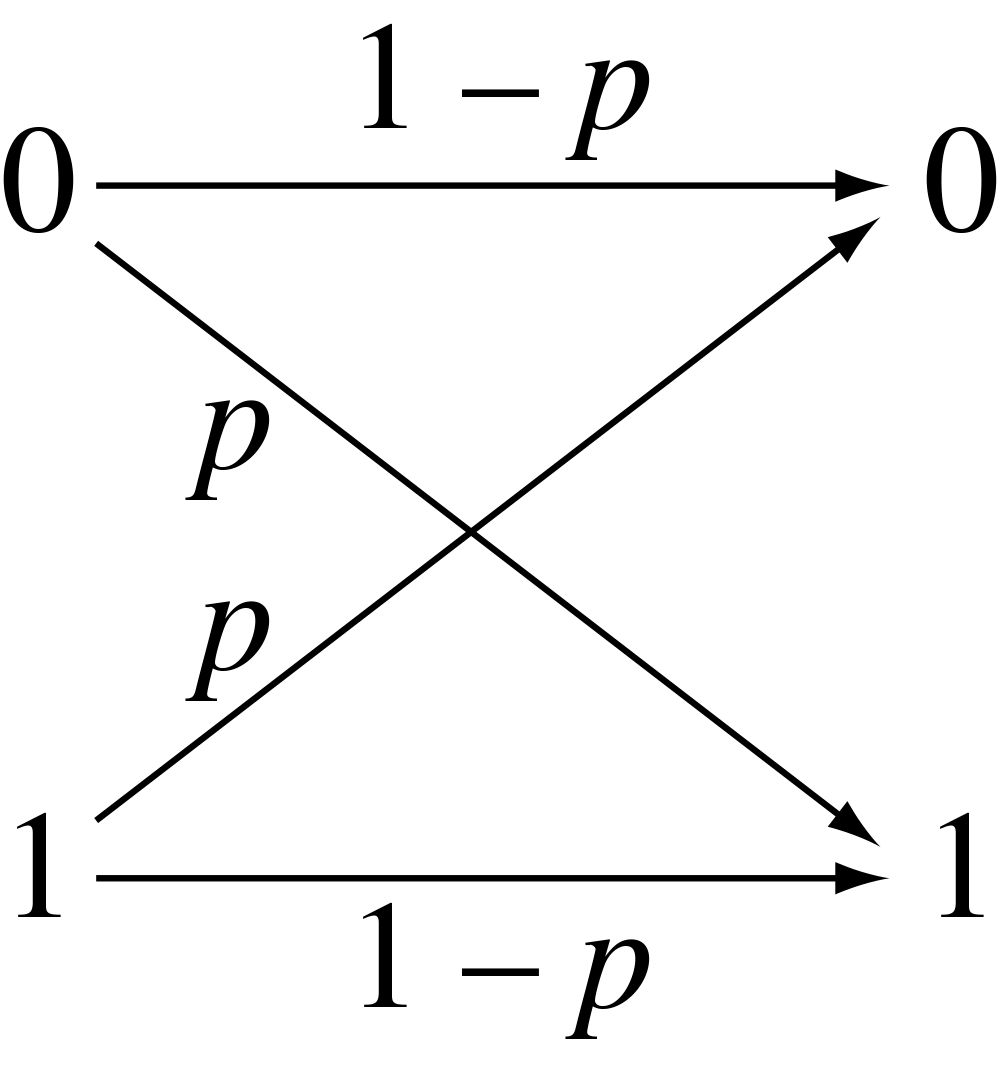
\includegraphics[width=0.3\linewidth]{figures/BSC.png}}
\caption{Το δυαδικό συμμετρικό κανάλι}
\label{fig:BSC channel}
\end{figure}

Αν υποθέσουμε πως το κανάλι είναι \textit{δυαδικό συμμετρικό} (\en{Binary Symmetric Channel - BSC}) κανάλι όπως στο Σχήμα \ref{fig:BSC channel}, η πιθανότητα να συμβεί σφάλμα σε οποιαδήποτε από τις $n$ θέσεις είναι η ίδια - $p$. Προκύπτει πως, υπάρχουν $2^n-1$ διαφορετικά μη-μηδενικά πρότυπα σφάλματος. 

Για την ανίχνευση σφαλμάτων, ο αποκωδικοποιητής υπολογίζει τις παρακάτω $n$-άδες στο $\mathbb{F}_2$:

\begin{equation}
\mathbf{s} = \left(s_0, s_1, \cdots, s_{n-k-1}\right) = \mathbf{r}\cdot\mathbf{H^T}
\label{eq:syndrome formation}
\end{equation}

Το διάνυσμα $\mathbf{s}$ καλείται \textit{σύνδρομο} του $\mathbf{r}$ \cite{ryan2009channel}. Σύμφωνα με την εξίσωση \ref{eq:syndrome formation} και όσα έχουν ήδη αναφερθεί, το ληφθέν διάνυσμα θα είναι κωδικολέξη του $C$ ανν $\mathbf{s}=0$. Σε αντίθετη περίπτωση το ληφθέν διάνυσμα δεν είναι κωδική λέξη και περιέχει \textit{σφάλματα μετάδοσης}.

Στην περίπτωση που ισχύει $\mathbf{s}=0$, ο αποκωδικοποιητής θεωρεί το ληφθέν διάνυσμα κωδικολέξη του $C$ χωρίς σφάλματα. Ωστόσο, στην περίπτωση που το $\mathbf{r}$ ανήκει στο κωδικό βιβλίο του $C$ αλλά διαφέρει από την κωδική λέξη που στάλθηκε $\mathbf{v}$, ο αποκωδικοποιητής διαπράττει \textit{σφάλμα αποκωδικοποίησης}. Αυτό συμβαίνει στην περίπτωση που το πρότυπο σφάλματος $\mathbf{e}$ ταυτίζεται με μία κωδική λέξη και καλείται \textit{μη-ανιχνεύσιμο} πρότυπο σφάλματος. Υπάρχουν $2^k-1$ μη-ανιχνεύσιμα πρότυπα σφάλματος \cite{macwilliams1977theory}.

\subsection{Αποκωδικοποίηση}

Ένας από τους σκοπούς της χρήσης κωδικοποίησης είναι η αύξηση της Ευκλείδιας απόστασης μεταξύ των μεταδιδόμενων σημάτων και κατά συνέπεια, η μείωση της πιθανότητας σφάλματος για δεδομένη ισχύ εκπομπής. Ισοδύναμα, απαιτείται η απόσταση \en{Hamming} μεταξύ των κωδικών λέξεων να είναι η μεγαλύτερη δυνατή. Καθώς ο υπολογισμός της απόστασης \en{Hamming} μεταξύ κάθε κωδικολέξης είναι πρακτικά αδύνατη διαδικασία, η σύγκριση της επίδοσης κωδίκων γίνεται με βάση την ελάχιστη απόσταση $d_{min}$ (ή με βάση το ελάχιστο βάρος $w_{min}$). Συνεπάγεται πως κώδικες με μεγαλύτερη $d_{min}$ έχουν συνήθως καλύτερες επιδόσεις \cite{proakis1994communication}.

Θεωρείται ο $C(n,k)$ γραμμικός \en{block} κώδικος με πίνακα ελέγχου ισοτιμίας $\mathbf{H}$, ελάχιστη απόσταση $d_{min}(C)$ και το ληφθέν διάνυσμα στο δέκτη, $\mathbf{r}$. Επιγραμματικά αναφέρεται πως, για αποκωδικοποίηση \textit{μέγιστης πιθανοφάνειας} (\en{maximum-likelihood decoding - MLD}), η απόφαση για τη μεταδιδόμενη κωδικολέξη λαμβάνεται με βάση τη μεγιστοποίηση της υπο-συνθήκη πιθανότητας $P(\mathbf{r}\mid\mathbf{v})$. Για το κανάλι \en{BSC} του Σχήματος \ref{fig:BSC channel}, αυτό ισοδυναμεί με τον υπολογισμό της απόστασης μεταξύ του $\mathbf{r}$ και κάθε κωδικής λέξης $\mathbf{v}$ και την επιλογή της κωδικής λέξης που ελαχιστοποιεί την απόσταση αυτή. Αυτός ο τρόπος αποκωδικοποίησης ονομάζεται \textit{κοντινότερου γείτονα} (\en{nearest-neighbor}) και αποτελεί αποκωδικοποίηση πλήρους \textit{διόρθωσης σφαλμάτων} (\en{complete error-correction}).

Η συγκεκριμένη μέθοδος αποκωδικοποίησης απαιτεί $2^k$ υπολογισμούς της απόστασης \en{Hamming}. Συνεπώς είναι αδύνατον να υλοποιηθεί πρακτικά. Στη συνέχεια θα δειχθούν μέθοδοι που χαρακτηρίζονται ως μη-πλήρους διόρθωσης σφαλμάτων, για να πετύχουν καλές επιδόσεις και ραγδαία μείωση της πολυπλοκότητας \cite{ryan2009channel}.

\subsection{Πολυπλοκότητα}

Τέλος, αναφορικά με την πολυπλοκότητα, αναφέρεται πως ο ορισμός της έννοιας της πολυπλοκότητας προσεγγίζεται δύσκολα. Ήδη από τη αναπαράσταση ενός γραμμικού \en{block} κώδικα, φαίνεται πως η πολυπλοκότητα περιγραφής (το ποσό μνήμης που χρειάζεται για να αποθηκευτεί ενάς κώδικας), είναι το πολύ $\min\langle Rn^2, \left(1-R\right)n^2\rangle$ \en{bits}, όπου $R$ ο ρυθμός του κώδικα. Επίσης όπως αναφέρθηκε ήδη, η κωδικοποίηση (αποτύπωση του μηνύματος πληροφορίας σε κωδική λέξη) οπώς προκύπτει από την εξίσωση \ref{eq:codeword formation}, γίνεται σε τετραγωνικό χρόνο $\mathcal{O}(n^2)$ \cite{richardson2008modern}.

Η πολυπλοκότητα αποκωδικοποίησης \en{MLD} σε ένα κανάλι \en{BSC} έχει αναλυθεί από τον \en{Berlekamp} κ.α. \cite{berlekamp1978inherent}. Αποδεικνύεται πως η \en{MLD} αποκωδικοποίηση είναι \en{NP-complete}, συνεπώς είναι απίθανο το \en{coding scheme} ενός γραμμικού \en{block} κώδικα να έχει πολυωνυμική πολυπλοκότητα \cite{bruck1990hardness}.


